61. Суммарная длина перегородок в клетчатом прямоугольнике $4\times5$ на рисунке равна 31. Чему равна суммарная длина перегородок в прямоугольнике $12\times50?$
\begin{center}
\begin{figure}[ht!]
\center{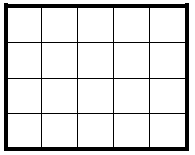
\includegraphics[scale=0.35]{12.png}}
\end{figure}
\end{center}

ewpage

oindent62. Суммарная длина перегородок в клетчатом прямоугольнике $4\times5$ на рисунке равна 31. Чему равна суммарная длина перегородок в прямоугольнике $40\times15?$
\begin{center}
\begin{figure}[ht!]
\center{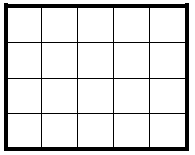
\includegraphics[scale=0.35]{12.png}}
\end{figure}
\end{center}
